%Para este capítulo se usará la abreviatura "cam".
\chapter{Conexión por caminos}
\label{cam}
La idea de conexión desarrollada en el capítulo anterior parece razonable, en el sentido de que un conjunto es conexo si no podemos realizar un ``corte limpio'' en dos piezas del conjunto.

No obstante, también parece razonable pensar que un conjunto será conexo si puedo ir andando de un lado a otro del mismo sin tener que dar saltos. Una aproximación a esta idea puede ser la conexión por poligonales, sin embargo, no parece lo suficientemente adecuada, ya que una circunferencia no es conexa por poligonales, pero en la mente humana está la idea de ir dando vueltas en círculos siguiendo el trazado de la circunferencia. Para formalizar esta idea nace la conexión por caminos.
\section{Generalidades sobre caminos}
Comenzamos definiendo lo que será el ingrediente estrella de este capítulo, los caminos.
\begin{defi}[Camino]
	Un \tbi{camino} en un espacio topológico $(\X,\T)$ es una aplicación continua $\sigma:[a,b]\to\X$. A los puntos $\sigma(a)$ y $\sigma(b)$ se les llama \tbi{extremos} del camino.
	
	En general, se dirá que $\sigma$ es un camino que conecta a sus extremos.
\end{defi}
Antes de meternos en harina hay que recordar estamos trabajando en espacios topológicos, es decir, aquí la intuición no vale de mucho.
\begin{obs}[Caminos densos]
	Cuando uno se imagina un camino, se imagina que la imagen del camino es una curva suave que no hace cosas demasiado extrañas, sin embargo la imagen de un camino puede ser densa en el plano. Este es el caso de la \tbi{curva de peano}, que no estudiaremos en estas notas.
\end{obs}
Al fin y al cabo los caminos no son más que parametrizaciones de subconjuntos de un espacio $\X$. Por esta razón, en ocasiones nos interesará considerar varios caminos (parametrizaciones) con la misma imagen o \tbi{traza}. A raiz de este problema emergen las llamadas ``reparametrizaciones''
\begin{obs}[Reparametrización]
	contenidos...
\end{obs}
Otro problema importante es el de ``yuxtaponer'' o ``pegar'' caminos, es decir, si tenemos un camino que termina en un extremo y otro que empieza en ese mismo extremo, queremos definir un camino cuya traza sea la unión de las trazas de ambos caminos. A continuación presentamos un procedimiento para resolver este problema.
\begin{exa}[Pegado de caminos]
	contenidos...
\end{exa}
\section{Conexión por caminos}
Comenzamos definiendo la noción de conexión por caminos.
\begin{defi}[Conexo por caminos]
	Un espacio $\X$ se dice \tbi[conexo!por caminos]{conexo por caminos} si para cualesquiera dos puntos de $\X$ hay un camino en $\X$ que los conecta.
\end{defi}
Una de las incógnitas que nos surgen al plantearnos una nueva noción de cualquier cosa es si esta es más fuerte o más débil que la que teníamos antes. En este caso, la conexión por caminos es más fuerte que la conexión ``a palo seco''.
\begin{prop}[Caminos y conexión]
	Si $\X$ es conexo por caminos, entonces $\X$ es conexo.
\end{prop}
\begin{proof}
	Evidentemente, si $\X$ es conexo por caminos podemos fijar un $x_0\in X$ y escribir $\X$ como $\X=\bigcup_{x\in\X}\Tr(\sigma_x)$, donde $\Tr(\sigma_x)$ denota a la traza del camino que conecta $x_0$ con $x$. Como los caminos son conexos por ser la imagen continua de un intervalo, la familia de conjuntos que conforma la unión es una familia de conexos, además, una familia de conexos cuya intersección contiene al menos a $x_0$. Luego, por el teorema del pivote $\X$ es conexo.
\end{proof}
Hay numerosos contraejemplos para ver que el recíproco no se cumple, veamos uno de ellos con todo detalle.
\begin{exa}[Seno del topólogo]
	contenidos...
\end{exa}
Una de esas cosas que nos hace volver a creer en la especie humana son los teoremas bonitos. Y el siguiente, que es un análogo del teorema del pivote para la conexión por caminos, lo es sin duda alguna.
\begin{theo}[Teorema del pivote]
	Sea $\{A_i\}_{i\in I}$ una familia de conexos por caminos con intersección no vacía. Entonces se verifica que la unión de la familia es conexa por caminos.
\end{theo}
\begin{proof}
	Sea $p$ un punto de la unión de la familia, luego habrá un índice $i_0$ para el cual $p\in A_{i_0}$, Además, como la intersección de la familia es no vacía, habrá un punto $a$ que esté en todos los miembros de la familia, en particular en $A_{i_0}$.
	
	Como $A_{i_0}$ es conexo por caminos habrá un camino $\sigma$ que conecte $p$ y $a$. Tomando otro punto $q$ en la unión de la familia, habrá un índice $i_1$ tal que $q\in A_{i_1}$. Como $a\in A_{i_1}$ y $A_{i_1}$ es conexo por caminos, habrá un camino $\tau$ que conecte $a$ con $q$.
	
	Pegando $\sigma$ y $\tau$ conseguimos un camino que une $p$ y $q$, y, como la elección de estos dos es arbitraria, hemos terminado.
\end{proof}
\section{Componentes conexas por caminos}
En esta sección estudiaremos el concepto análogo al de las componentes conexas, pero para esta noción de conexión.
\begin{defi}[Componente conexa por caminos]
	Dado un punto $x$ de un espacio $\X$ se dice que un conjunto $\Co(x)$ que contiene a $x$ es una \tbi[componente conexa!por caminos]{componente conexa por caminos} de $x$ si $\Co(x)$ es un conjunto conexo ``maximal''. Es decir, el mayor conjunto conexo por caminos que contiene a $x$. En general se dirá que $\Co(x)$ es una componente conexa si lo es de alguno de sus puntos (luego de todos, como veremos más adelante).
\end{defi}
A continuación demostramos resultados análogos a los ya demostrados para la noción de conexión, haciendo hincapié en las relaciones entre las dos nociones.
\begin{lem}[Caracterización conjuntista]
	contenidos...
\end{lem}
\begin{proof}
	contenidos...
\end{proof}
\section{Local--conexión por caminos}
\begin{defi}[Localmente conexo por caminos]
	Un espacio $\X$ se dice \tbi{localmente conexo por caminos} si todo punto del espacio tiene una base de entornos conexos por caminos.
\end{defi}
Sin más dilación vamos a caracterizar, como hicimos en el capítulo anterior, la versión local de esta noción de conexión.
\begin{lem}[Caracterización]
	Las siguientes afirmaciones son equivalentes.
	\begin{enumerate}
		\item $\X$ es localmente conexo por caminos.
		\item Las componentes conexas por caminos de de los abiertos de $\X$ son abiertas.
		\item Cada punto de $\X$ tiene una base de entornos conexos por caminos y abiertos.
	\end{enumerate}
\end{lem}
\begin{proof} Realicemos nuestro círculo virtuoso habitual.
\end{proof}
Esta vez, la local--conexión por caminos nos aporta algo más, una condición suficiente para que un conjunto sea conexo por caminos.
\begin{prop}[Condición suficiente]
	Si $\X$ es conexo y localmente conexo por caminos, entonces $\X$ es conexo por caminos.
\end{prop}
\begin{proof}
	contenidos...
\end{proof}
\section{Comportamiento topológico}
Presentamos esta vez, para variar, la tabla--resumen al comienzo la sección. A continuación iremos estudiando caso por caso el comportamiento topológico de las diferentes nociones de conexión introducidas en este capítulo.
\begin{table}[H]
	\centering
	\begin{tabular}{c|c|c|c|c|}
		\cline{2-5}
		\multicolumn{1}{l|}{}                                                                                  & \multicolumn{1}{l|}{\textbf{Subespacios}}                             & \multicolumn{1}{l|}{\textbf{Cociente}} & \multicolumn{1}{l|}{\textbf{Producto}} & \multicolumn{1}{l|}{\textbf{Suma}} \\ \hline
		\multicolumn{1}{|c|}{\textbf{\begin{tabular}[c]{@{}c@{}}Conexo por\\ caminos\end{tabular}}}            & No                                                                    & Sí                                     & Sí                                     & No                                 \\ \hline
		\multicolumn{1}{|c|}{\textbf{\begin{tabular}[c]{@{}c@{}}Localmente conexo\\ por caminos\end{tabular}}} & \begin{tabular}[c]{@{}c@{}}Sí, en el caso \\ de abiertos\end{tabular} & Sí                                     & Sí                                     & Sí                                 \\ \hline
	\end{tabular}
	\caption{Tabla resumen de conexión por caminos}
	\label{Tabla_conexion_caminos}
\end{table}
Veamos aquí de forma condensada las pintorescas relaciones entre las distintas formas de ver la conexión.
\begin{figure}[h!]
	\centering
	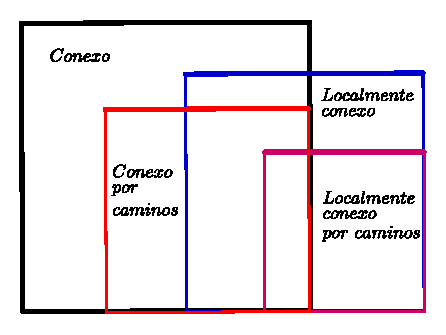
\includegraphics[scale = 1]{img/Comparacion_conexion}
	\caption{Ilustración de las relaciones entre las diferentes nociones de conexión.}
\end{figure}
